\documentclass{article}
\usepackage[margin=1in]{geometry}
\usepackage{array}
\usepackage{longtable}
\usepackage{booktabs}
\usepackage{graphicx}
\usepackage{float}
\begin{document}
\footnotesize
\setlength{\tabcolsep}{4pt}
\renewcommand{\arraystretch}{0.9}
\section*{S7.1 Body}

\section*{S7.1}
\renewcommand{\arraystretch}{1.1}
\setlength{\tabcolsep}{6pt}
\begin{table}[H]
\centering
\begin{tabular}{lrrrrl}
\hline
\multicolumn{6}{l}{\textit{S7.1}} \\
\hline
Test & Stat & $p$ & df & Dist & Reject \\
\hline
Box-Pierce Q & 13.430 & 0.098 & 8 & Chi2 & No \\
\multicolumn{6}{l}{\footnotesize{H0: No serial correlation up to lag 8}} \\
Ljung-Box Q & 14.266 & 0.075 & 8 & Chi2 & No \\
\multicolumn{6}{l}{\footnotesize{H0: No serial correlation up to lag 8}} \\
\hline
\end{tabular}
\end{table}

\clearpage
\section*{S7.2a Body}

\section*{S7.2(A)}
\begin{figure}[H]
\centering
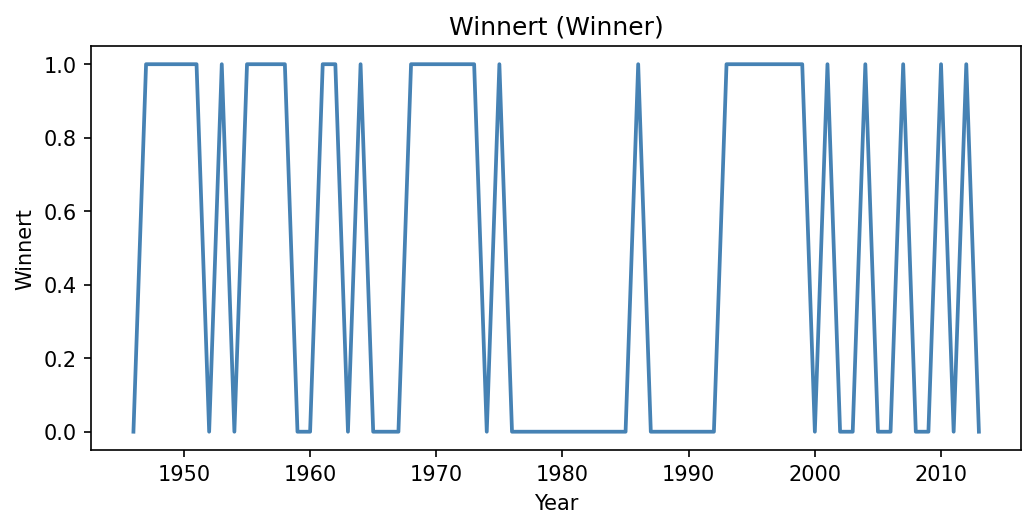
\includegraphics[width=0.95\linewidth]{S7.2A_time_series.png}
\caption{Time-series plot of Winnert (Winner)}
\end{figure}
\begin{figure}[H]
\centering
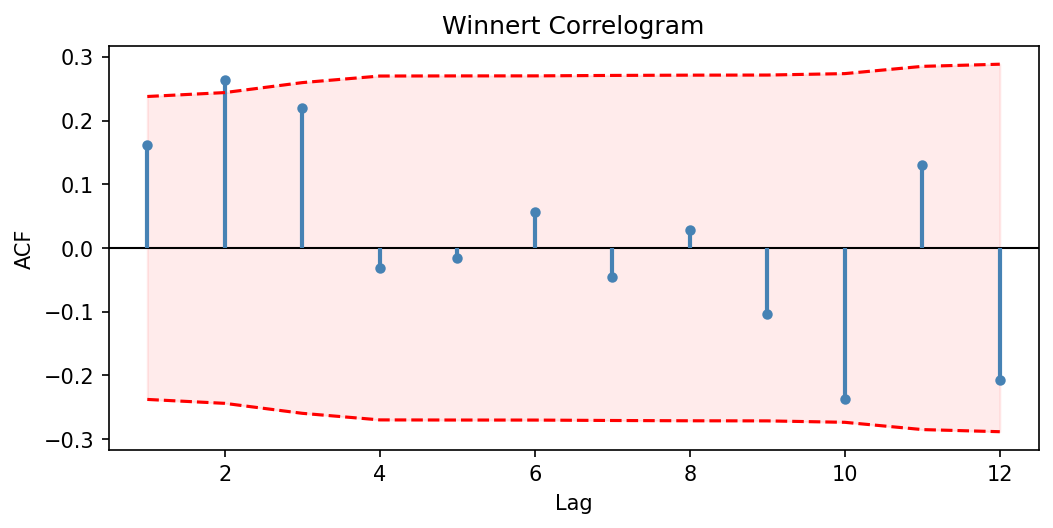
\includegraphics[width=0.95\linewidth]{S7.2A_correlogram.png}
\caption{Sample correlogram of Winnert with Bartlett 95\% bands (MA(0))}
\end{figure}

\clearpage
\section*{S7.2b Body}

\section*{S7.2(B)}
We test the null that the Winner series is white noise using the Ljung--Box test with $m=4$. 
The test statistic is $Q_{LB} = 10.503$ with $\chi^2_4$ reference distribution and 
$p$-value $= 0.033$. 
At the 5\% level, we 
\textbf{reject} the null of white noise.

\clearpage
\section*{S7.2c Body}

\section*{S7.2(C)}
\begin{figure}[H]
\centering
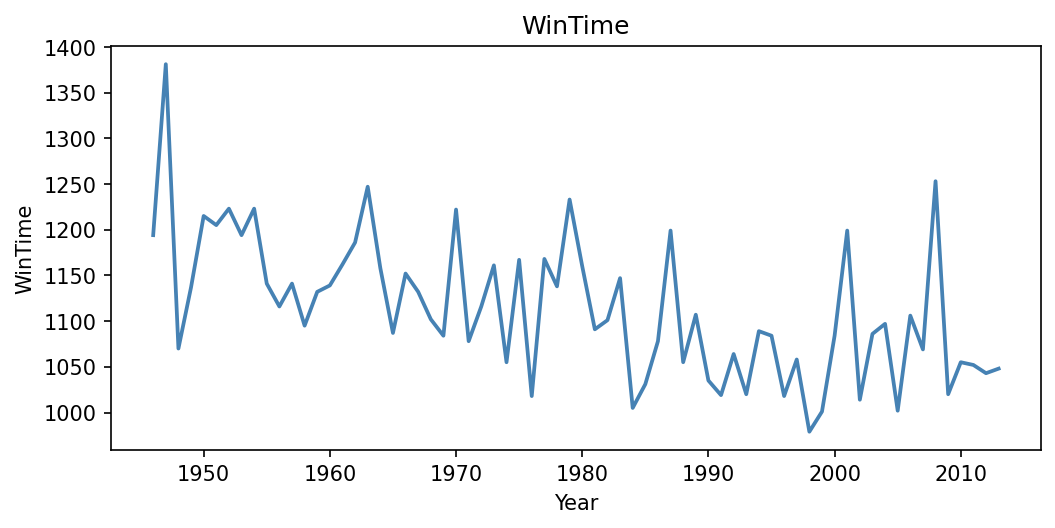
\includegraphics[width=0.95\linewidth]{S7.2C_wintime.png}
\caption{Time-series plot of WinTime}
\end{figure}
\begin{figure}[H]
\centering
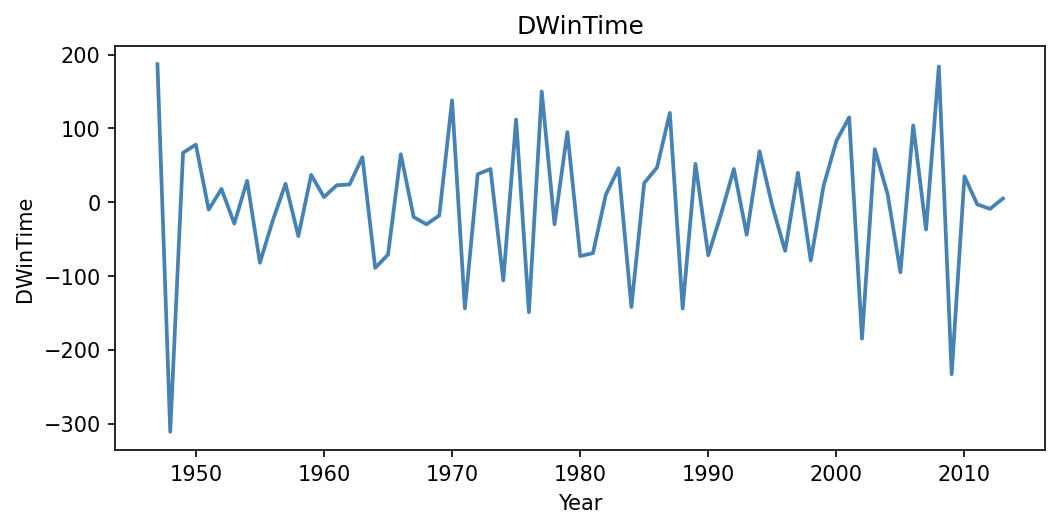
\includegraphics[width=0.95\linewidth]{S7.2C_dwintime.png}
\caption{Time-series plot of DWinTime}
\end{figure}
\begin{figure}[H]
\centering
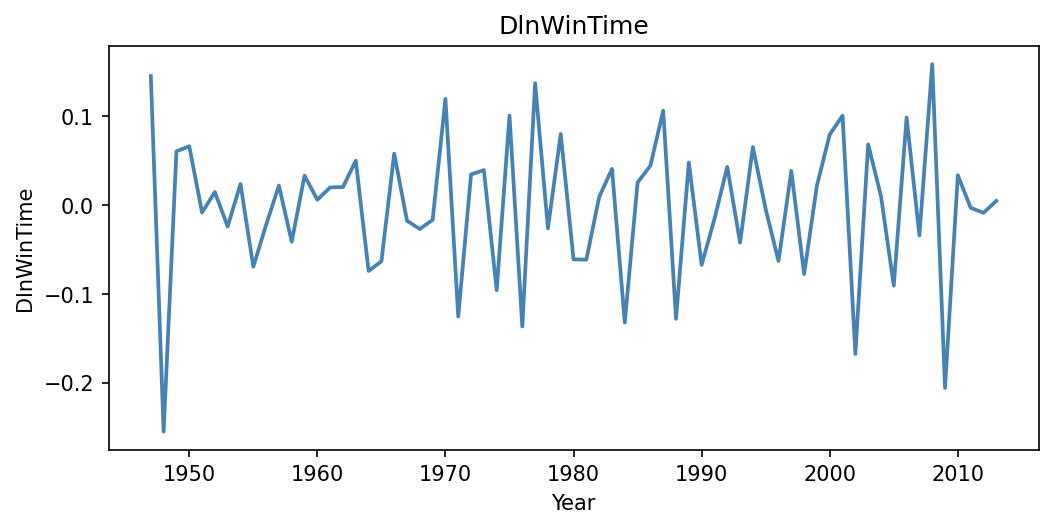
\includegraphics[width=0.95\linewidth]{S7.2C_dlnwintime.png}
\caption{Time-series plot of DlnWinTime}
\end{figure}
WinTime shows moderate long-run variation with no obvious deterministic trend; year-to-year changes appear noisy. 
The first difference DWinTime fluctuates around zero with occasional spikes, suggesting short-run shocks. 
The log-difference DlnWinTime similarly centers near zero and compresses large swings, indicating proportionate changes are small and mean-reverting.
\begin{figure}[H]
\centering
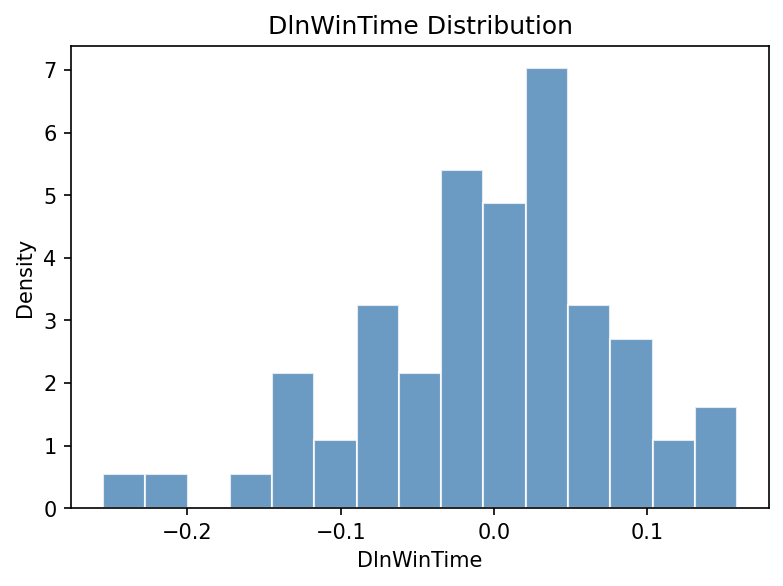
\includegraphics[width=0.75\linewidth]{S7.2C_dlnwintime_dist.png}
\caption{Distribution of DlnWinTime (histogram, density)}
\end{figure}

\clearpage
\section*{S7.2e Body}

\section*{S7.2(E)}
\begin{figure}[H]
\centering
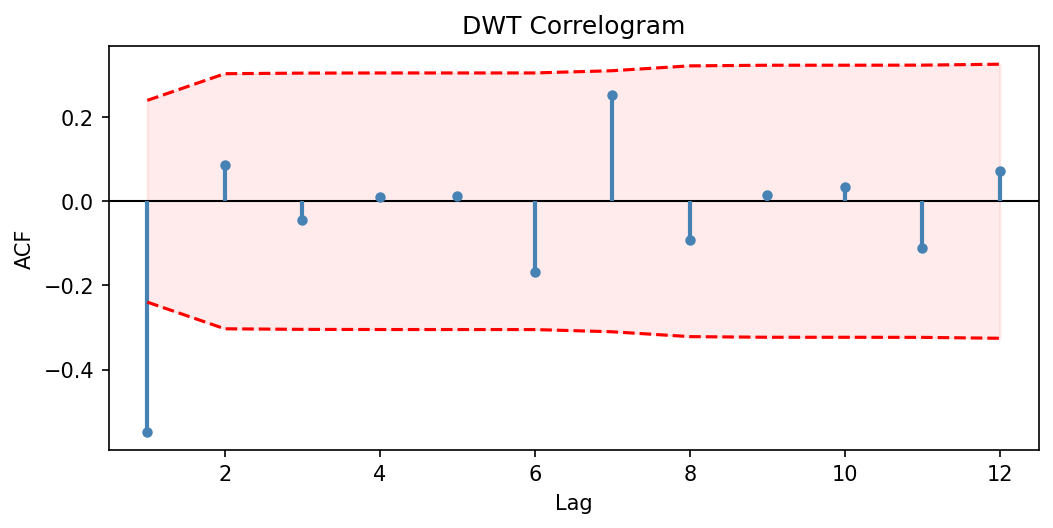
\includegraphics[width=0.95\linewidth]{S7.2E_correlogram.png}
\caption{Sample correlogram of DWT (first difference of WinTime) with Bartlett 95\% bands (MA(0))}
\end{figure}

\end{document}